\documentclass{tufte-book}%[a4paper,twoside]
% See https://github.com/Tufte-LaTeX/tufte-latex/blob/master/sample-book.tex for details

\title{Alice in Bitcoinland}
\author{Gigi}
\publisher{Do I Really Need a Publisher}

% Packages
\usepackage{lipsum}
\usepackage{booktabs}
\usepackage{graphicx}
\setkeys{Gin}{width=\linewidth,totalheight=\textheight,keepaspectratio}
\graphicspath{{graphics/}}

%%
% Just some sample text
\usepackage{lipsum}

%%
% For nicely typeset tabular material
\usepackage{booktabs}

%%
% Bibliography stuff: Biber, BibTex, BibLatex
%\usepackage[autostyle]{csquotes}
% \usepackage[
    % backend=biber,
    % style=authoryear-icomp,
    % sortlocale=de_DE,
    % natbib=true,
    % url=false,
    % doi=true,
    % eprint=false
% ]{biblatex}
% \usepackage[backend=biber]{biblatex}
\usepackage{natbib}
\bibliographystyle{abbrvnat}

%%
% Hyperlinks
\usepackage{hyperref}

%%
% For graphics / images
\usepackage{graphicx}
\setkeys{Gin}{width=\linewidth,totalheight=\textheight,keepaspectratio}
\graphicspath{{graphics/}}

% The fancyvrb package lets us customize the formatting of verbatim
% environments.  We use a slightly smaller font.
\usepackage{fancyvrb}
\fvset{fontsize=\normalsize}

%%
% Prints argument within hanging parentheses (i.e., parentheses that take
% up no horizontal space).  Useful in tabular environments.
\newcommand{\hangp}[1]{\makebox[0pt][r]{(}#1\makebox[0pt][l]{)}}

%%
% Prints an asterisk that takes up no horizontal space.
% Useful in tabular environments.
\newcommand{\hangstar}{\makebox[0pt][l]{*}}

%%
% Prints a trailing space in a smart way.
\usepackage{xspace}

% Prints the month name (e.g., January) and the year (e.g., 2008)
\newcommand{\monthyear}{%
  \ifcase\month\or January\or February\or March\or April\or May\or June\or
  July\or August\or September\or October\or November\or
  December\fi\space\number\year
}


% Prints an epigraph and speaker in sans serif, all-caps type.
\newcommand{\openepigraph}[2]{%
  %\sffamily\fontsize{14}{16}\selectfont
  \begin{fullwidth}
  \sffamily\large
  \begin{doublespace}
  \noindent\allcaps{#1}\\% epigraph
  \noindent\allcaps{#2}% author
  \end{doublespace}
  \end{fullwidth}
}

% Inserts a blank page
\newcommand{\blankpage}{\newpage\hbox{}\thispagestyle{empty}\newpage}

\usepackage{units}

% Typesets the font size, leading, and measure in the form of 10/12x26 pc.
\newcommand{\measure}[3]{#1/#2$\times$\unit[#3]{pc}}

% Macros for typesetting the documentation
\newcommand{\hlred}[1]{\textcolor{Maroon}{#1}}% prints in red
\newcommand{\hangleft}[1]{\makebox[0pt][r]{#1}}
\newcommand{\hairsp}{\hspace{1pt}}% hair space
\newcommand{\hquad}{\hskip0.5em\relax}% half quad space
\newcommand{\TODO}{\textcolor{red}{\bf TODO!}\xspace}
\newcommand{\na}{\quad--}% used in tables for N/A cells
\providecommand{\XeLaTeX}{X\lower.5ex\hbox{\kern-0.15em\reflectbox{E}}\kern-0.1em\LaTeX}
\newcommand{\tXeLaTeX}{\XeLaTeX\index{XeLaTeX@\protect\XeLaTeX}}
% \index{\texttt{\textbackslash xyz}@\hangleft{\texttt{\textbackslash}}\texttt{xyz}}
\newcommand{\tuftebs}{\symbol{'134}}% a backslash in tt type in OT1/T1
\newcommand{\doccmdnoindex}[2][]{\texttt{\tuftebs#2}}% command name -- adds backslash automatically (and doesn't add cmd to the index)
\newcommand{\doccmddef}[2][]{%
  \hlred{\texttt{\tuftebs#2}}\label{cmd:#2}%
  \ifthenelse{\isempty{#1}}%
    {% add the command to the index
      \index{#2 command@\protect\hangleft{\texttt{\tuftebs}}\texttt{#2}}% command name
    }%
    {% add the command and package to the index
      \index{#2 command@\protect\hangleft{\texttt{\tuftebs}}\texttt{#2} (\texttt{#1} package)}% command name
      \index{#1 package@\texttt{#1} package}\index{packages!#1@\texttt{#1}}% package name
    }%
}% command name -- adds backslash automatically
\newcommand{\doccmd}[2][]{%
  \texttt{\tuftebs#2}%
  \ifthenelse{\isempty{#1}}%
    {% add the command to the index
      \index{#2 command@\protect\hangleft{\texttt{\tuftebs}}\texttt{#2}}% command name
    }%
    {% add the command and package to the index
      \index{#2 command@\protect\hangleft{\texttt{\tuftebs}}\texttt{#2} (\texttt{#1} package)}% command name
      \index{#1 package@\texttt{#1} package}\index{packages!#1@\texttt{#1}}% package name
    }%
}% command name -- adds backslash automatically
\newcommand{\docopt}[1]{\ensuremath{\langle}\textrm{\textit{#1}}\ensuremath{\rangle}}% optional command argument
\newcommand{\docarg}[1]{\textrm{\textit{#1}}}% (required) command argument
\newenvironment{docspec}{\begin{quotation}\ttfamily\parskip0pt\parindent0pt\ignorespaces}{\end{quotation}}% command specification environment
\newcommand{\docenv}[1]{\texttt{#1}\index{#1 environment@\texttt{#1} environment}\index{environments!#1@\texttt{#1}}}% environment name
\newcommand{\docenvdef}[1]{\hlred{\texttt{#1}}\label{env:#1}\index{#1 environment@\texttt{#1} environment}\index{environments!#1@\texttt{#1}}}% environment name
\newcommand{\docpkg}[1]{\texttt{#1}\index{#1 package@\texttt{#1} package}\index{packages!#1@\texttt{#1}}}% package name
\newcommand{\doccls}[1]{\texttt{#1}}% document class name
\newcommand{\docclsopt}[1]{\texttt{#1}\index{#1 class option@\texttt{#1} class option}\index{class options!#1@\texttt{#1}}}% document class option name
\newcommand{\docclsoptdef}[1]{\hlred{\texttt{#1}}\label{clsopt:#1}\index{#1 class option@\texttt{#1} class option}\index{class options!#1@\texttt{#1}}}% document class option name defined
\newcommand{\docmsg}[2]{\bigskip\begin{fullwidth}\noindent\ttfamily#1\end{fullwidth}\medskip\par\noindent#2}
\newcommand{\docfilehook}[2]{\texttt{#1}\index{file hooks!#2}\index{#1@\texttt{#1}}}
\newcommand{\doccounter}[1]{\texttt{#1}\index{#1 counter@\texttt{#1} counter}}

% Generates the index
\usepackage{makeidx}
\makeindex

%%
% Chapter/Lesson Quotes
\makeatletter
\renewcommand{\@chapapp}{}% Not necessary...
\newenvironment{chapquote}[2][4em]
  {\setlength{\@tempdima}{#1}%
   \def\chapquote@author{#2}%
   \parshape 1 \@tempdima \dimexpr\textwidth-2\@tempdima\relax%
   \itshape}
  %{\par\normalfont\hfill--\ \chapquote@author\hspace*{\@tempdima}\par\bigskip}
  \par\bigskip
\makeatother

\begin{document}

\frontmatter

\maketitle

\cleardoublepage


%%
% Start the main matter (normal chapters)
\mainmatter

\part*{21 Lessons}

\chapter*{Introduction}
\label{ch:introduction}

\begin{chapquote}{Lewis Carroll, \textit{Alice in Wonderland}}
``But I don’t want to go among mad people,'' Alice remarked. ``Oh, you can’t
help that,'' said the Cat: ``we’re all mad here. I’m mad. You’re mad.'' ``How do
you know I’m mad?'' said Alice. ``You must be,'' said the Cat, ``or you wouldn’t
have come here.''
\end{chapquote}

In October 2018, Arjun Balaji asked the innocuous question,
\textit{What have you learned from Bitcoin?} After trying to answer this
question in a short tweet, and failing miserably, I realized that the things
I've learned are far too numerous to answer quickly, if at all.

The things I've learned are, obviously, about Bitcoin - or at least related to
it. However, while some of the inner workings of Bitcoin are explained, the
following lessons are not an explanation of how Bitcoin works or what it is,
they might, however, help to explore some of the things Bitcoin touches:
philosophical questions, economic realities, and technological innovations.

\begin{center}
  
\includegraphics[width=7cm]{assets/images/the-tweet.png}
\end{center}

The \textit{21 Lessons} are structured in bundles of seven, resulting in three
chapters. Each chapter looks at Bitcoin through a different lens, extracting
what lessons can be learned by inspecting this strange network from a different
angle.

\paragraph{\hyperref[ch:philosophy]{Chapter 1}}{explores the philosophical
teachings of Bitcoin. The interplay of immutability and change, the concept of
true scarcity, Bitcoin's immaculate conception, the problem of identity, the
contradiction of replication and locality, the power of free speech, and the
limits of knowledge.
}

\paragraph{\hyperref[ch:economics]{Chapter 2}}{explores the economic teachings
of Bitcoin. Lessons about financial ignorance, inflation, value, money and the
history of money, fractional reserve banking, and how Bitcoin is re-introducing
sound money in a sly, roundabout way.}

\paragraph{\hyperref[ch:technology]{Chapter 3}}{explores some of the lessons
learned by examining the technology of Bitcoin.  Why there is strength in
numbers, reflections on trust, why telling time takes work, how moving slowly
and not breaking things is a feature and not a bug, what Bitcoin's creation can
tell us about privacy, why cypherpunks write code (and not laws), and what
metaphors might be useful to explore Bitcoin's future.}

~

Each lesson contains several quotes and links throughout the text. If an idea is
worth exploring in more detail, you can follow the links to related works in the
footnotes or in the bibliography.

Even though some prior knowledge about Bitcoin is beneficial, I hope that these
lessons can be digested by any curious reader. While some relate to each other,
each lesson should be able to stand on its own and can be read independently. I
did my best to shy away from technical jargon, even though some domain-specific
vocabulary is unavoidable.

I hope that my writing serves as inspiration for others to dig beneath the
surface and examine some of the deeper questions Bitcoin raises. My own
inspiration came from a multitude of authors and content creators to all of whom
I am eternally grateful.

Last but not least: my goal in writing this is not to convince you of anything.
My goal is to make you think, and show you that there is way more to Bitcoin
than meets the eye. I can’t even tell you what Bitcoin is or what Bitcoin will
teach you. You will have to find that out for yourself.

\begin{samepage}\begin{quotation}
\enquote{After this, there is no turning back. You take the blue pill --- the
story ends, you wake up in your bed and believe whatever you want to
believe. You take the red pill\footnote{the \textit{orange} pill} --- you stay in Wonderland, and I show
you how deep the rabbit hole goes.}
\flushright -- Morpheus
\end{quotation}\end{samepage}

\begin{figure}
  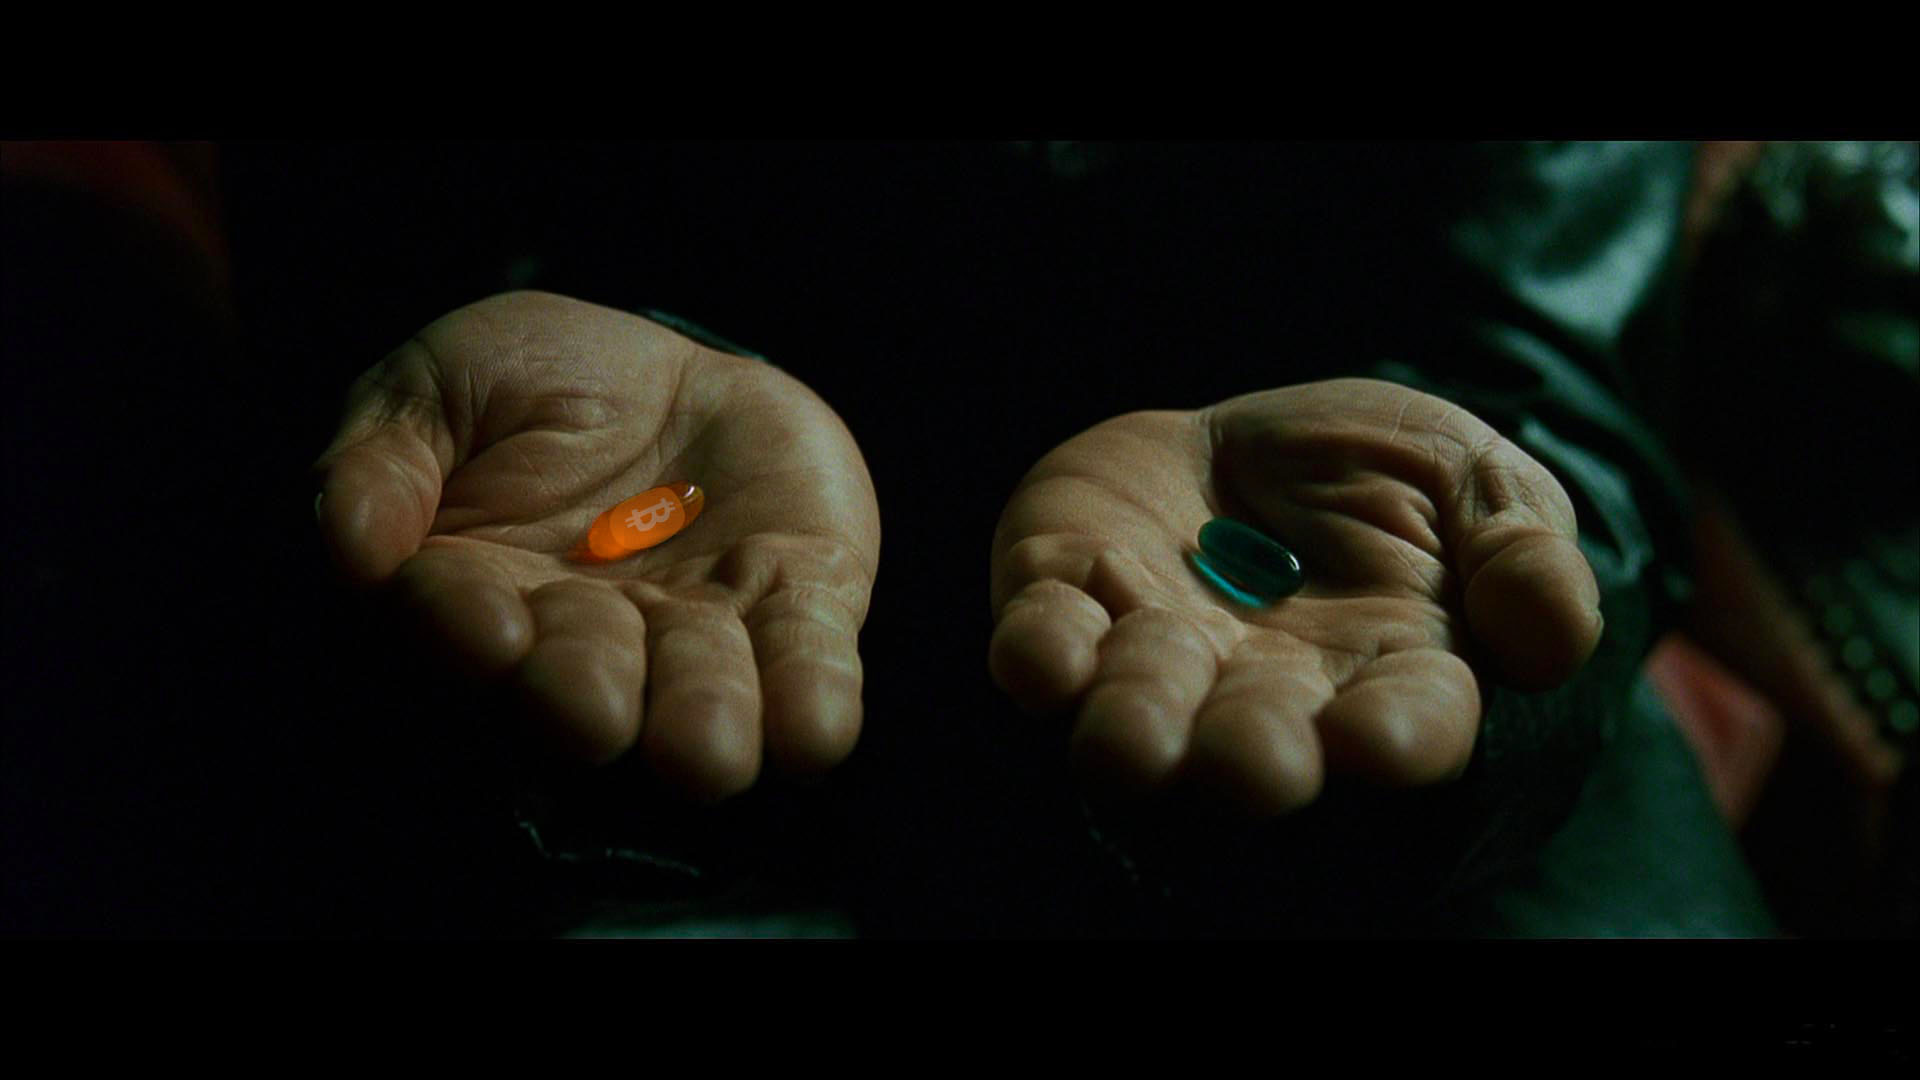
\includegraphics{assets/images/bitcoin-orange-pill.jpg}
  \caption*{Remember: All I'm offering is the truth. Nothing more.}
  \label{fig:bitcoin-orange-pill}
\end{figure}

%
% [Morpheus]: https://en.wikipedia.org/wiki/Red_pill_and_blue_pill#The_Matrix_(1999)
% [this question]: https://twitter.com/arjunblj/status/1050073234719293440
%
% <!-- Internal -->
% [chapter1]: {{ 'bitcoin/lessons/ch1-00-philosophy' | absolute_url }}
% [chapter2]: {{ 'bitcoin/lessons/ch2-00-economics' | absolute_url }}
% [chapter3]: {{ 'bitcoin/lessons/ch3-00-technology' | absolute_url }}
%
% <!-- Wikipedia -->
% [alice]: https://en.wikipedia.org/wiki/Alice%27s_Adventures_in_Wonderland
% [carroll]: https://en.wikipedia.org/wiki/Lewis_Carroll

\part{Philosophy}
\label{ch:philosophy}

% \blockquote{
% The mouse looked at her rather inquisitively, and seemed to her to wink with one
% of its little eyes, but it said nothing.
% }
%
% \newthought{Looking at Bitcoin} superficially, one might conclude that it is slow, wasteful,
% unnecessarily redundant, and overly paranoid. Looking at Bitcoin inquisitively,
% one might find out that things are not as they seem at first glance.

Bitcoin has a way of taking your assumptions and turning them on their heads.
After a while, just when you were about to get comfortable again, Bitcoin will
smash through the wall like a bull in a china shop and shatter your assumptions
once more.

\begin{figure}
  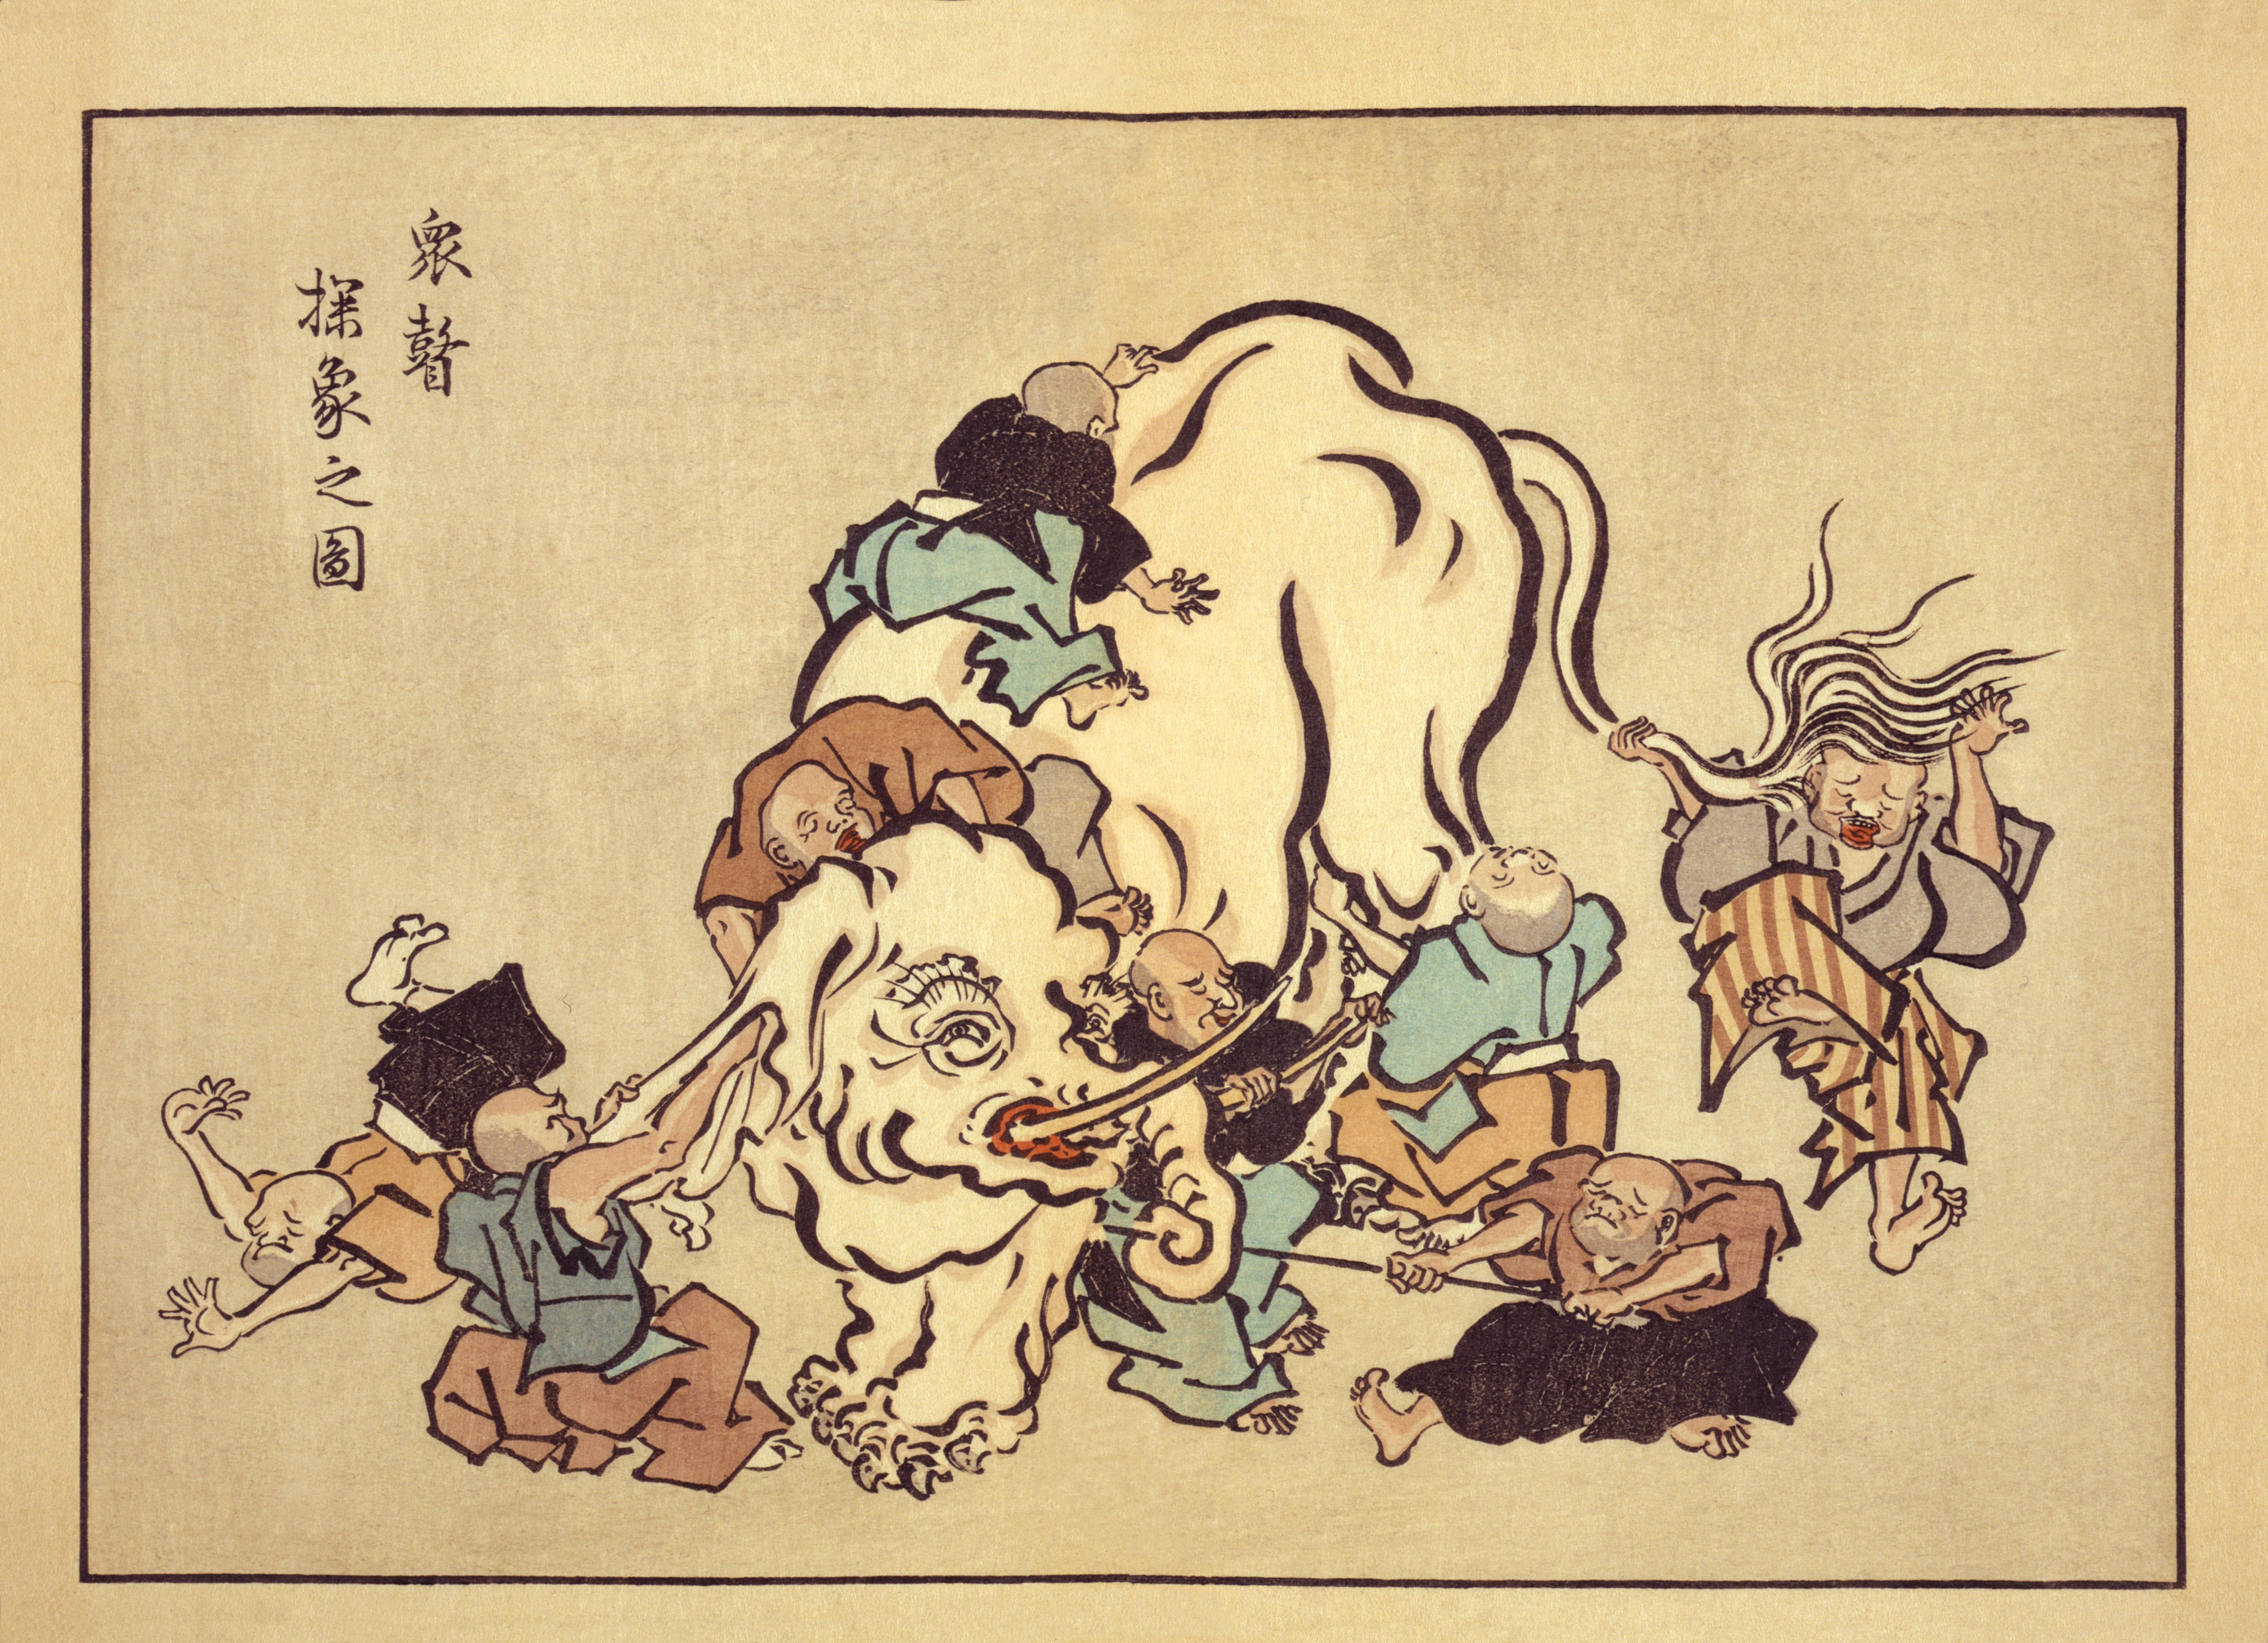
\includegraphics{assets/images/blind-monks.jpg}
  \caption{Blind monks examining the Bitcoin bull}
  \label{fig:blind-monks}
\end{figure}

Bitcoin is a child of many disciplines. Like blind monks examining an elephant,
everyone who approaches this novel technology does so from a different angle.
And everyone will come to different conclusions about the nature of the beast.

The following lessons are about some of my assumptions which Bitcoin shattered,
and the conclusions I arrived at. Philosophical questions of immutability,
scarcity, locality, and identity are explored in the first four lessons.

TODO: Lesson List
% 

Lesson 5 explores how Bitcoin's origin story is not only fascinating but
absolutely essential for a leaderless system. The last two lessons of this
chapter explore the power of free speech and the limits of our individual
knowledge, reflected by the surprising depth of the Bitcoin rabbit hole.

I hope that you will find the world of Bitcoin as educational, fascinating and
entertaining as I did and still do. I invite you to follow the white rabbit and
explore the depths of this rabbit hole. Now hold on to your pocket watch, pop
down, and enjoy the fall.

\chapter{Immutability and Change}
\label{les:1}

\begin{chapquote}{Alice}
\enquote{I wonder if I've been changed in the night. Let me think. Was I the same when I
got up this morning? I almost think I can remember feeling a little different.
But if I'm not the same, the next question is `Who in the world am I?' Ah,
that's the great puzzle!}
\end{chapquote}

Bitcoin is inherently hard to describe. It is a \textit{new thing}, and any
attempt to draw a comparison to previous concepts -- be it by calling
it digital gold or the internet of money -- is bound to fall short of
the whole. Whatever your favorite analogy might be, two aspects of
Bitcoin are absolutely essential: decentralization and immutability.

\paragraph{}
One way to think about Bitcoin is as an automated social contract\footnote{Hasu,
Unpacking Bitcoin's Social Contract~\cite{social-contract}}. The software is
just one piece of the puzzle, and hoping to change Bitcoin by changing the
software is an exercise in futility. One would have to convince the rest of the
network to adopt the changes, which is more a psychological effort than a
software engineering one.

\paragraph{}
The following might sound absurd at first, like so many other things in
this space, but I believe that it is profoundly true nonetheless: You
won't change Bitcoin, but Bitcoin will change you.

\begin{quotation}\begin{samepage}
\enquote{Bitcoin will change us more than we will change it.}
\begin{flushright} -- Marty Bent\footnote{Tales From the Crypt~\cite{tftc21}}
\end{flushright}\end{samepage}\end{quotation}

It took me a long time to realize the profundity of this. Since Bitcoin
is just software and all of it is open-source, you can simply change
things at will, right? Wrong. \textit{Very} wrong. Unsurprisingly, Bitcoin's
creator knew this all too well.

\begin{quotation}\begin{samepage}
\enquote{The nature of Bitcoin is such that once version 0.1 was released, the core
design was set in stone for the rest of its lifetime.}
\begin{flushright} -- Satoshi Nakamoto\footnote{BitcoinTalk forum post: `Re:
Transactions and Scripts\ldots'~\cite{satoshi-set-in-stone}}
\end{flushright}\end{samepage}\end{quotation}

Many people have attempted to change Bitcoin's nature. So far all of
them have failed. While there is an endless sea of forks and altcoins,
the Bitcoin network still does its thing, just as it did when the first
node went online. The altcoins won't matter in the long run. The forks
will eventually starve to death. Bitcoin is what matters. As long as our
fundamental understanding of mathematics and/or physics doesn't change,
the Bitcoin honeybadger will continue to not care.

\begin{quotation}\begin{samepage}
\enquote{Bitcoin is the first example of a new form of life. It lives and
breathes on the internet. It lives because it can pay people to keep
it alive. [\ldots] It can't be changed. It can't be argued with. It
can't be tampered with. It can't be corrupted. It can't be stopped.
[\ldots] If nuclear war destroyed half of our planet, it would continue
to live, uncorrupted.}
\begin{flushright} -- Ralph Merkle\footnote{DAOs, Democracy and
Governance,~\cite{merkle-dao}}
\end{flushright}\end{samepage}\end{quotation}

The heartbeat of the Bitcoin network will outlast all of ours.

~

Realizing the above changed me way more than the past blocks of the Bitcoin
blockchain ever will. It changed my time preference, my understanding of
economics, my political views, and so much more. Hell, it is even changing
people's diets\footnote{Inside the World of the Bitcoin
Carnivores,~\cite{carnivores}}. If all of this sounds crazy to you, you're in
good company. All of this is crazy, and yet it is happening.

~

\paragraph{Bitcoin taught me that it won't change. I will.}

% ---
%
% #### Through the Looking-Glass
%
% - [Bitcoin's Gravity: How idea-value feedback loops are pulling people in][gravity]
% - [Lesson 18: Move slowly and don't break things][lesson18]
%
% #### Down the Rabbit Hole
%
% - [Unpacking Bitcoin's Social Contract][automated social contract]: A framework for skeptics by Hasu
% - [DAOs, Democracy and Governance][Ralph Merkle] by Ralph C. Merkle
% - [Marty's Bent][bent]: A daily newsletter highlighting signal in Bitcoin by Marty Bent
% - [Technical Discussion on Bitcoin's Transactions and Scripts][Satoshi Nakamoto] by Satoshi Nakamoto, Gavin Andresen, and others
% - [Inside the World of the Bitcoin Carnivores][carnivores]: Why a small community of Bitcoin users is eating meat exclusively by Jordan Pearson
% - [Tales From the Crypt][tftc] hosted by Marty Bent
%
% <!-- Internal -->
% [gravity]: 
% [lesson18]: {{ 'bitcoin/lessons/ch3-18-move-slowly-and-dont-break-things' | absolute_url }}
%
% <!-- Further Reading -->
% [automated social contract]: https://medium.com/@hasufly/bitcoins-social-contract-1f8b05ee24a9
% [carnivores]: https://motherboard.vice.com/en_us/article/ne74nw/inside-the-world-of-the-bitcoin-carnivores
% [tftc]: https://tftc.io/tales-from-the-crypt/
% [bent]: https://tftc.io/martys-bent/
%
% <!-- Quotes -->
% [Ralph Merkle]: http://merkle.com/papers/DAOdemocracyDraft.pdf
% [Satoshi Nakamoto]: https://bitcointalk.org/index.php?topic=195.msg1611#msg1611
%
% <!-- Twitter People -->
% [Marty Bent]: https://twitter.com/martybent
%
% <!-- Wikipedia -->
% [alice]: https://en.wikipedia.org/wiki/Alice%27s_Adventures_in_Wonderland
% [carroll]: https://en.wikipedia.org/wiki/Lewis_Carroll


\chapter{ The Scarcity of Scarcity}
\label{les:2}

\begin{chapquote}{Alice}
That's quite enough - I hope I sha'n't grow any more...
\end{chapquote}

In general, the advance of technology seems to make things more abundant. More
and more people are able to enjoy what previously have been luxurious goods.
Soon, we will all live like kings. Most of us already do. As Peter Diamandis
wrote in Abundance\cite{abundance}: ``Technology is a resource-liberating
mechanism. It can make the once scarce the now abundant.''

Bitcoin, an advanced technology in itself, breaks this trend and creates
a new commodity which is truly scarce. Some even argue that it is one of
the scarcest things in the universe. The supply can't be inflated, no
matter how much effort one chooses to expend towards creating more.

\begin{chapquote}{\cite{bitcoinstandard-pres}}
``Only two things are genuinely scarce: time and
bitcoin.''
\end{chapquote}

Paradoxically, it does so by a mechanism of copying. Transactions are
broadcast, blocks are propagated, the distributed ledger is --- well,
you guessed it --- distributed. All of these are just fancy words for
copying. Heck, Bitcoin even copies itself onto as many computers as it
can, by incentivizing individual people to run full nodes and mine new
blocks.

All of this duplication wonderfully works together in a concerted effort
to produce scarcity.

In a time of abundance, Bitcoin taught me what real scarcity is.

% ---
%
% #### Through the Looking-Glass
%
% - [Lesson 14: Sound money][lesson14]
%
% #### Down the Rabbit Hole
%
% - [The Bitcoin Standard: The Decentralized Alternative to Central Banking][bitcoin-standard]
% - [Abundance: The Future Is Better Than You Think][Abundance] by Peter Diamandis
% - [Presentation on The Bitcoin Standard][bitcoin-standard-presentation] by Saifedean Ammous
% - [Modeling Bitcoin's Value with Scarcity][planb-scarcity] by PlanB
% - 🎧 [Misir Mahmudov on the Scarcity of Time & Bitcoin][tftc60] TFTC #60 hosted by Marty Bent
% - 🎧 [PlanB – Modelling Bitcoin's digital scarcity through stock-to-flow techniques][slp67] SLP #67 hosted by Stephan Livera
%
% <!-- Through the Looking-Glass -->
% [lesson14]: {{ 'bitcoin/lessons/ch2-14-sound-money' | absolute_url }}
%
% <!-- Down the Rabbit Hole -->
% [Abundance]: https://www.diamandis.com/abundance
% [bitcoin-standard]: http://amzn.to/2L95bJW
% [bitcoin-standard-presentation]: https://www.bayernlb.de/internet/media/de/ir/downloads_1/bayernlb_research/sonderpublikationen_1/bitcoin_munich_may_28.pdf
% [planb-scarcity]: https://medium.com/@100trillionUSD/modeling-bitcoins-value-with-scarcity-91fa0fc03e25
% [tftc60]: https://anchor.fm/tales-from-the-crypt/episodes/Tales-from-the-Crypt-60-Misir-Mahmudov-e3aibh
% [slp67]: https://stephanlivera.com/episode/67
%
% <!-- Wikipedia -->
% [alice]: https://en.wikipedia.org/wiki/Alice%27s_Adventures_in_Wonderland
% [carroll]: https://en.wikipedia.org/wiki/Lewis_Carroll

\chapter{The Problem of Identity}
\label{les:4}

\begin{chapquote}{Lewis Carroll, \textit{Alice in Wonderland}}
  \enquote{Who are you?} said the caterpillar.
\end{chapquote}

Nic Carter, in an homage to Thomas Nagel's treatment of the same
question in regards to a bat, wrote an excellent piece which discusses
the following question: What is it like to be a bitcoin? He
brilliantly shows that open, public blockchains in general, and Bitcoin
in particular, suffer from the same conundrum as the Ship of
Theseus: which Bitcoin is the real Bitcoin?

\begin{quotation}\begin{samepage}
\enquote{Consider just how little persistence Bitcoin's components have. The
entire codebase has been reworked, altered, and expanded such that it
barely resembles its original version. [...] The registry of who
owns what, the ledger itself, is virtually the only persistent trait
of the network [...]
To be considered truly leaderless, you must surrender the easy
solution of having an entity that can designate one chain as the
legitimate one.}
\begin{flushright} -- Nic Carter\footnote{Nic Carter, \textit{What is it like to be a bitcoin?} \cite{bitcoin-identity}}
\end{flushright}\end{samepage}\end{quotation}

It seems like the advancement of technology keeps forcing us to take
these philosophical questions seriously. Sooner or later, self-driving
cars will be faced with real-world versions of the trolley problem,
forcing them to make ethical decisions about whose lives do matter and
whose do not.

Cryptocurrencies, especially since the first contentious hard-fork,
force us to think about and agree upon the metaphysics of identity.
Interestingly, the two biggest examples we have so far have lead to two
different answers. On August 1, 2017, Bitcoin split into two camps. The
market decided that the unaltered chain is the original Bitcoin. One
year earlier, on October 25, 2016, Ethereum split into two camps. The
market decided that the \textit{altered} chain is the original Ethereum.

If properly decentralized, the questions posed by the \textit{Ship of Theseus}
will have to be answered in perpetuity for as long as these networks of
value-transfer exist.

\paragraph{Bitcoin taught me that decentralization contradicts identity.}

% ---
%
% #### Down the Rabbit Hole
%
% - [What Is It Like to be a Bat?][in regards to a bat] by Thomas Nagel
% - [What is it like to be a bitcoin?] by Nic Carter
% - [Ship of Theseus], [trolley problem] on Wikipedia
%
% [in regards to a bat]: https://en.wikipedia.org/wiki/What_Is_it_Like_to_Be_a_Bat%3F
% [What is it like to be a bitcoin?]: https://medium.com/s/story/what-is-it-like-to-be-a-bitcoin-56109f3e6753
% [Ship of Theseus]: https://en.wikipedia.org/wiki/Ship_of_Theseus
% [trolley problem]: https://en.wikipedia.org/wiki/Trolley_problem
%
% <!-- Wikipedia -->
% [alice]: https://en.wikipedia.org/wiki/Alice%27s_Adventures_in_Wonderland
% [carroll]: https://en.wikipedia.org/wiki/Lewis_Carroll


\chapter{Economics}
\label{ch:economics}

\begin{chapquote}{Lewis Carroll, \textit{Alice in Wonderland}}
``A large rose tree stood near the entrance of the garden: the roses on it were
white, but there were three gardeners at it, busily painting them red. This
Alice thought a very curious thing...''
\end{chapquote}

\newthought{Money doesn’t grow on trees.} To believe that it does is foolish, and our
parents make sure that we know about that by repeating this saying like a
mantra. We are encouraged to use money wisely, to not spend it frivolously,
and to save it in good times to help us through the bad. Money, after all,
does not grow on trees.

Bitcoin taught me more about money than I ever thought I would need to know.
Through it, I was forced to explore the history of money, banking, various
schools of economic thought, and many other things. The quest to understand
Bitcoin lead me down a plethora of paths, some of which I try to explore in
this series.

In the first seven lessons some of the philosophical questions Bitcoin touches
on were discussed. The next seven lessons will take a closer look at money and
economics.

\TODO{Lesson List}
% 

Again, I will only be able to scratch the surface. Bitcoin is not only
ambitious, but also broad and deep in scope, making it impossible to cover all
relevant topics in a single lesson, essay, article, or book. I  doubt if it is
even possible at all.

\newthought{Bitcoin is a new form of money}, which makes learning about
economics paramount to understanding it. Dealing with the nature of human action
and the interactions of economic agents, economics is probably one of the
largest and fuzziest pieces of the Bitcoin puzzle.

Again, these lessons are an exploration of the various things I have learned
from Bitcoin. They are a personal reflection of my journey down the rabbit hole.
Having no background in economics, I am definitely out of my comfort zone and
especially aware that any understanding I might have is incomplete. I will do my
best to outline what I have learned, even at the risk of making a fool out of
myself. After all, I am still trying to answer the question: ``What have you
learned from Bitcoin?''

\begin{marginfigure}%
  
\includegraphics{assets/images/the-tweet.png}
  \caption{What have you learned from Bitcoin?}
  \label{fig:tweet}
\end{marginfigure}

After seven lessons examined through the lens of philosophy, let’s use the lens
of economics to look at seven more. Economy class is all I can offer this time.
Final destination: \textit{sound money}.

% [the question]: https://twitter.com/arjunblj/status/1050073234719293440

\part{Technology}
\label{ch:technology}

\begin{chapquote}{Lewis Carroll, \textit{Alice in Wonderland}}
``Now, I'll manage better this time'' she said to herself, and began by taking
the little golden key, and unlocking the door that led into the garden
\end{chapquote}

\newthought{Golden keys}, clocks which only work by chance, races to solve
strange riddles, and builders that don't have faces or names. What sounds like
fairy tales from Wonderland is daily business in the world of Bitcoin.

As we explored in [Chapter 2][chapter2], large parts of the current financial
system are systematically broken. Like Alice, we can only hope to manage better
this time. But, thanks to a pseudonymous inventor, we have incredibly
sophisticated technology to support us this time around: Bitcoin.

Solving problems in a radically decentralized and adversarial environment
requires unique solutions. What would otherwise be trivial problems to solve
are everything but in this strange world of nodes. Bitcoin relies on strong
cryptography for most solutions, at least if looked at through the lens of
technology. Just how strong this cryptography is will be explored in one of the
following lessons.

\newthought{Cryptography} is what Bitcoin uses to remove trust in authorities.
Instead of relying on centralized institutions, the system relies on the final
authority of our universe: physics. Some grains of trust still remain, however.
We will examine these grains in the second lesson of this chapter.

% 

The last couple of lessons explore the ethos of technological development in
Bitcoin, which is arguably as important as the technology itself. Bitcoin is not
the next shiny app on your phone. It is the foundation of a new economic
reality, which is why Bitcoin should be treated as nuclear-grade financial
software.

Where are we in this financial, societal, and technological revolution? Networks
and technologies of the past may serve as metaphors for Bitcoins future, which
are explored in the last lesson of this chapter.

Once more, strap in and enjoy the ride. Like all exponential technologies, we
are about to go parabolic.

\addpart{Conclusion}
\label{ch:conclusion}

\begin{chapquote}{Lewis Carroll, \textit{Alice in Wonderland}}
``Begin at the beginning'' the King said, very gravely, ``and go on till you
come to the end: then stop.''
\end{chapquote}

\textit{As mentioned in the beginning}, I think that any answer to the
question *“What have you learned from Bitcoin?”* will always be incomplete. The
symbiosis of what can be seen as multiple living systems -- Bitcoin, the
technosphere, and economics -- is too intertwined, the topics too numerous, and
things are moving too fast to ever be fully understood by a single person.

Even without understanding it fully, and even with all its quirks and seeming
shortcomings, Bitcoin undoubtedly works. It keeps producing blocks roughly every
ten minutes and does so beautifully. The longer Bitcoin continues to work, the
more people will opt-in to use it.

\begin{quotation}
``It's true that things are beautiful when they work. Art is function.'' \flushright
-- Giannina Braschi
\end{quotation}

\textit{Bitcoin is a child of the internet}. It is growing exponentially,
blurring the lines between disciplines. It isn’t clear, for example, where the
realm of pure technology ends and where another realm begins. Even though
Bitcoin requires computers to function efficiently, computer science is not
sufficient to understand it. Bitcoin is not only borderless in regards to its
inner workings but also boundaryless in respect to academic disciplines.

Economics, politics, game theory, monetary history, network theory, finance,
cryptography, information theory, censorship, law and regulation, human
organization, psychology -- all these and more are areas of expertise which might
help in the quest of understanding how Bitcoin works and what Bitcoin is.

No single invention is responsible for its success. It is the combination of
multiple, previously unrelated pieces, glued together by game theoretical
incentives, which make up the revolution that is Bitcoin. The beautiful blend of
many disciplines is what makes Satoshi a genius.

\textit{Like every complex system}, Bitcoin has to make tradeoffs in terms
of efficiency, cost, security, and many other properties. Just like there is no
perfect solution to deriving a square from a circle, any solution to the
problems which Bitcoin tries to solve will always be imperfect as well.

% > “I don’t believe we shall ever have a good money again before we take the
% > thing out of the hands of government, that is, we can’t take it violently
% > out of the hands of government, all we can do is by some sly roundabout way
% > introduce something that they can’t stop.”
% > <cite>[Friedrich Hayek][sly roundabout way]</cite>

Bitcoin is the sly, roundabout way to re-introduce good money to the world. It
does so by placing a sovereign individual behind each node, just like Da Vinci
tried to solve the intractable problem of squaring a circle by placing the
Vitruvian Man in its center. Nodes effectively remove any concept of a center,
creating a system which is astonishingly antifragile and extremely hard to shut
down. Bitcoin lives, and its heartbeat will probably outlast all of ours.

I hope you have enjoyed these twenty-one lessons. Maybe the most important
lesson is that Bitcoin should be examined holistically, from multiple angles, if
one would like to have something approximating a complete picture. Just like
removing one part from a complex system destroys the whole, examining parts of
Bitcoin in isolation seems to taint the understanding of it. If only one person
strikes "blockchain" from her vocabulary and replaces it with "a chain of
blocks" I will die a happy man.

In any case, my journey continues. I plan to venture further down into the
depths of this rabbit hole, and I invite you to [tag along][dergigi] for the ride.

% <!-- Twitter -->
% [dergigi]: https://twitter.com/dergigi
%
% <!-- Internal -->
% [sly roundabout way]: https://youtu.be/EYhEDxFwFRU?t=1124
% [Giannina Braschi]: https://en.wikipedia.org/wiki/Braschi%27s_Empire_of_Dreams


\bibliography{main}

\end{document}
